%!TEX root = ../../master.tex

\section{Network Topology (Physical)}
The physical network topology of a KubeCloud is set up in a star-topology with the switch as the center of the cluster. Figure~\ref{fig:topology} illustrates this setup.

\begin{figure}[H]
    \centering
    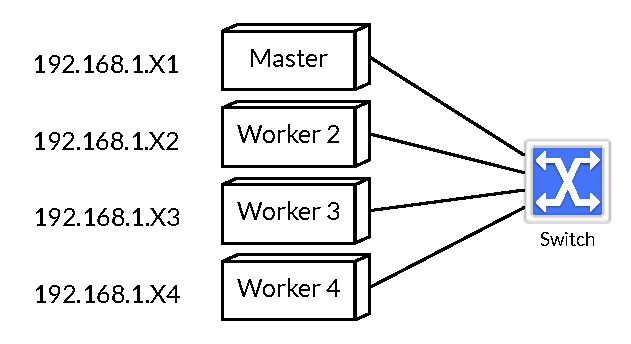
\includegraphics[width=6.5cm]{figures/raspberry_cluster_topology}
    \caption{Network Topology}
    \label{fig:topology}
\end{figure}

\noindent
The static IP convention in each KubeCloud cluster is depicted in Figure~\ref{fig:topology}. The static IP convention assumes clusters of four nodes with the last of the four octets representing a group number and the location of the node in the cluster. The first digit of the last octet determines the group number while the second digit determines the location. The location follows a convention of the master node being the topmost physical location. The following worker nodes and IPs are increasing downwards, e.g. group 1 will have the following nodes: 192.168.1.11 (Master), 192.168.1.12 (Worker 2), 192.168.1.13 (Worker 3), 192.168.1.14 (Worker 4). \\

\noindent
An alternative to static IPs is to use zero-configuration networking implementation such as Avahi. A test was conducted in the beginning of the project, but the stability of using Avahi was not satisfying in our case. Therefore, the static IP convention was chosen instead. Static IPs are rigid and can limit the number of nodes in a cluster following the naming convention, but stability was the crucial parameter. This way of configuring the IPs of the cluster allows for easily connecting the single cluster to the entire network of clusters used in the classroom. This decoupling of clusters allows for custom configuration of cluster sizes, which will be explained in the software section of this chapter. When putting it all together, the clusters are again set up in star-topology as depicted in Figure~\ref{fig:topology_overall}.

\begin{figure}[H]
    \centering
    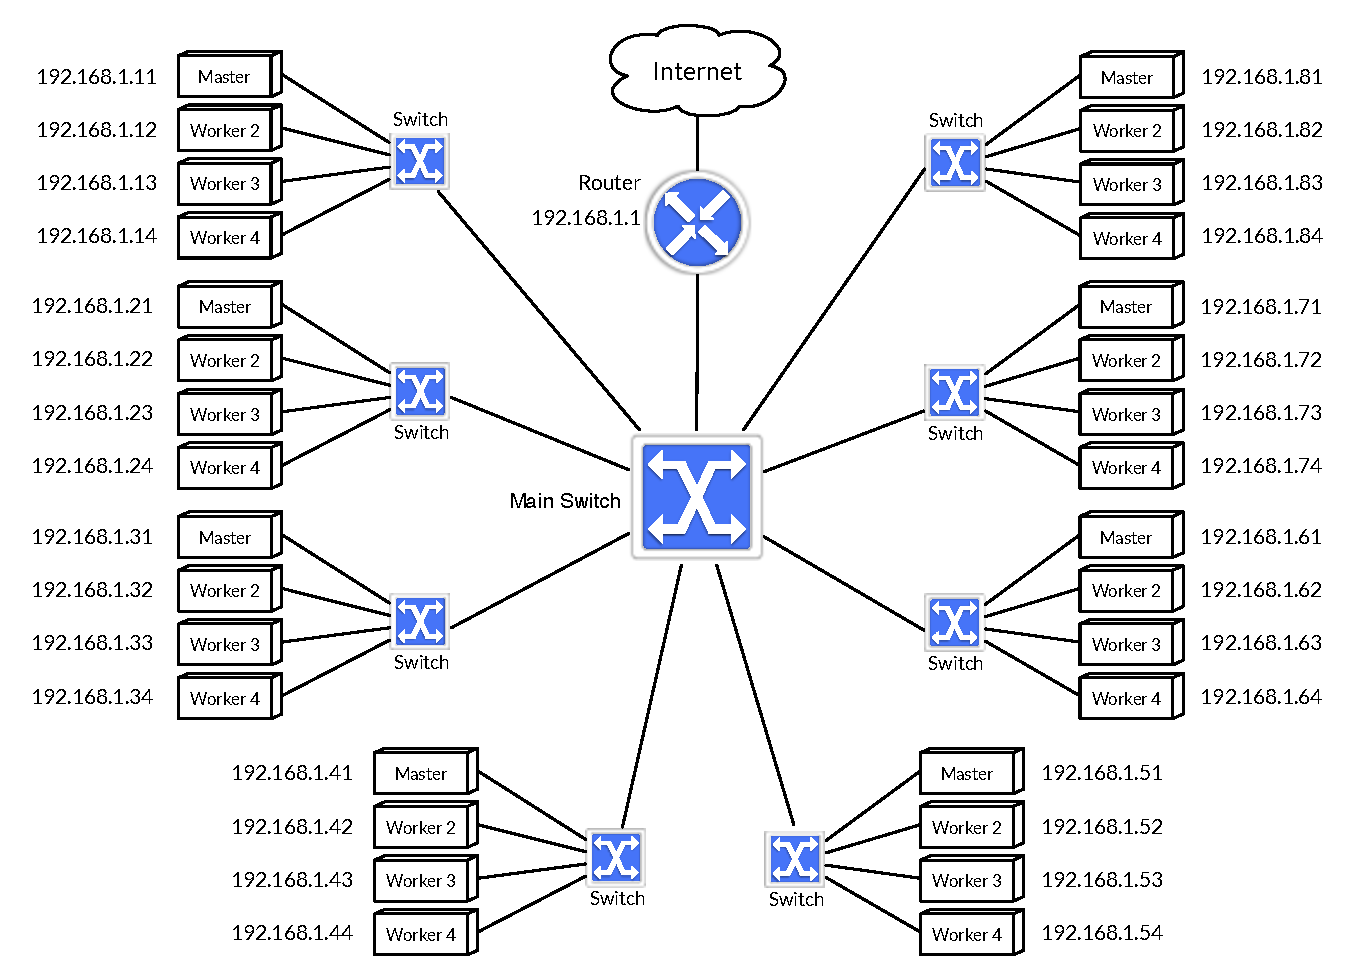
\includegraphics[width=\textwidth]{figures/overall_topology}
    \caption{Overall Network Topology}
    \label{fig:topology_overall}
\end{figure}

\noindent 
The router act as the gateway for the internet connection needed to access the Docker Hub repositories. 